%%%%%%%%%%%%%%%%%%%%%%%%%%%%%%%%%%%%%%%%%
% fphw Assignment
% LaTeX Template
% Version 1.0 (27/04/2019)
%
% This template originates from:
% https://www.LaTeXTemplates.com
%
% Authors:
% Class by Felipe Portales-Oliva (f.portales.oliva@gmail.com) with template 
% content and modifications by Vel (vel@LaTeXTemplates.com)
%
% Template (this file) License:
% CC BY-NC-SA 3.0 (http://creativecommons.org/licenses/by-nc-sa/3.0/)
%
%%%%%%%%%%%%%%%%%%%%%%%%%%%%%%%%%%%%%%%%%

%----------------------------------------------------------------------------------------
%	PACKAGES AND OTHER DOCUMENT CONFIGURATIONS
%----------------------------------------------------------------------------------------

\documentclass[
	12pt, % Default font size, values between 10pt-12pt are allowed
	%letterpaper, % Uncomment for US letter paper size
	%spanish, % Uncomment for Spanish
]{fphw}

% Template-specific packages
\usepackage[utf8]{inputenc} % Required for inputting international characters
\usepackage[T1]{fontenc} % Output font encoding for international characters
\usepackage{mathpazo} % Use the Palatino font

\usepackage{graphicx} % Required for including images

\usepackage{booktabs} % Required for better horizontal rules in tables

\usepackage{listings} % Required for insertion of code

\usepackage{enumerate} % To modify the enumerate environment

\usepackage[utf8]{inputenc}
\usepackage[LGR,T1]{fontenc}
\usepackage[english,greek]{babel}


%----------------------------------------------------------------------------------------
%	ASSIGNMENT INFORMATION
%----------------------------------------------------------------------------------------

\title{Προχωρημένα Θέματα Βάσεων Δεδομένων \\ Εξαμηνιαία Εργασία} % Assignment title


\author{Πέτρος Βιτάλης Α.Μ.: 03121117 \\ Κιμίνου Φραγκίσκα Α.Μ.: 03121009} % Student name

\date{Δεκέμβριος, 2025} % Due date

\institute{Εθνικό Μετσόβιο Πολυτεχνείο \\ Σχολή Ηλεκτρολόγων Μηχανικών και Μηχανικών Υπολογιστών \\ Τομέας Τεχνολογίας Πληροφορικής και Υπολογιστών \\ Εργαστήριο Βάσεων Γνώσεων και Δεδομένων} % Institute or school name

\class{Ακαδημαϊκό Έτος: 2025-2026 \\ Διδάσκων: Δημήτριος Τσουμάκος \\ Υπεύθυνος Εργαστηρίου: Νικόλαος Χαλβαντζής} % Course or class name

%----------------------------------------------------------------------------------------

\begin{document}

\maketitle % Output the assignment title, created automatically using the information in the custom commands above

%----------------------------------------------------------------------------------------
%	ASSIGNMENT CONTENT
%----------------------------------------------------------------------------------------

\selectlanguage{english}
\section*{Query 1}
\selectlanguage{greek}


\begin{problem}
	Να υλοποιηθεί το \selectlanguage{english}Query 1\selectlanguage{greek} χρησιμοποιώντας τα \selectlanguage{english}DataFrame\selectlanguage{greek} (με και χωρίς \selectlanguage{english}UDF\selectlanguage{greek}) και \selectlanguage{english}RDD APIs\selectlanguage{greek}. Να εκτελέσετε και τις δύο υλοποιήσεις με \selectlanguage{english}4 executors (1 core, 2GB memory)\selectlanguage{greek}. Υπάρχει διαφορά στην επίδοση μεταξύ των τριών υλοποιήσεων? Να σχολιάσετε τα ευρήματά σας.

\end{problem}
\begin{center}
	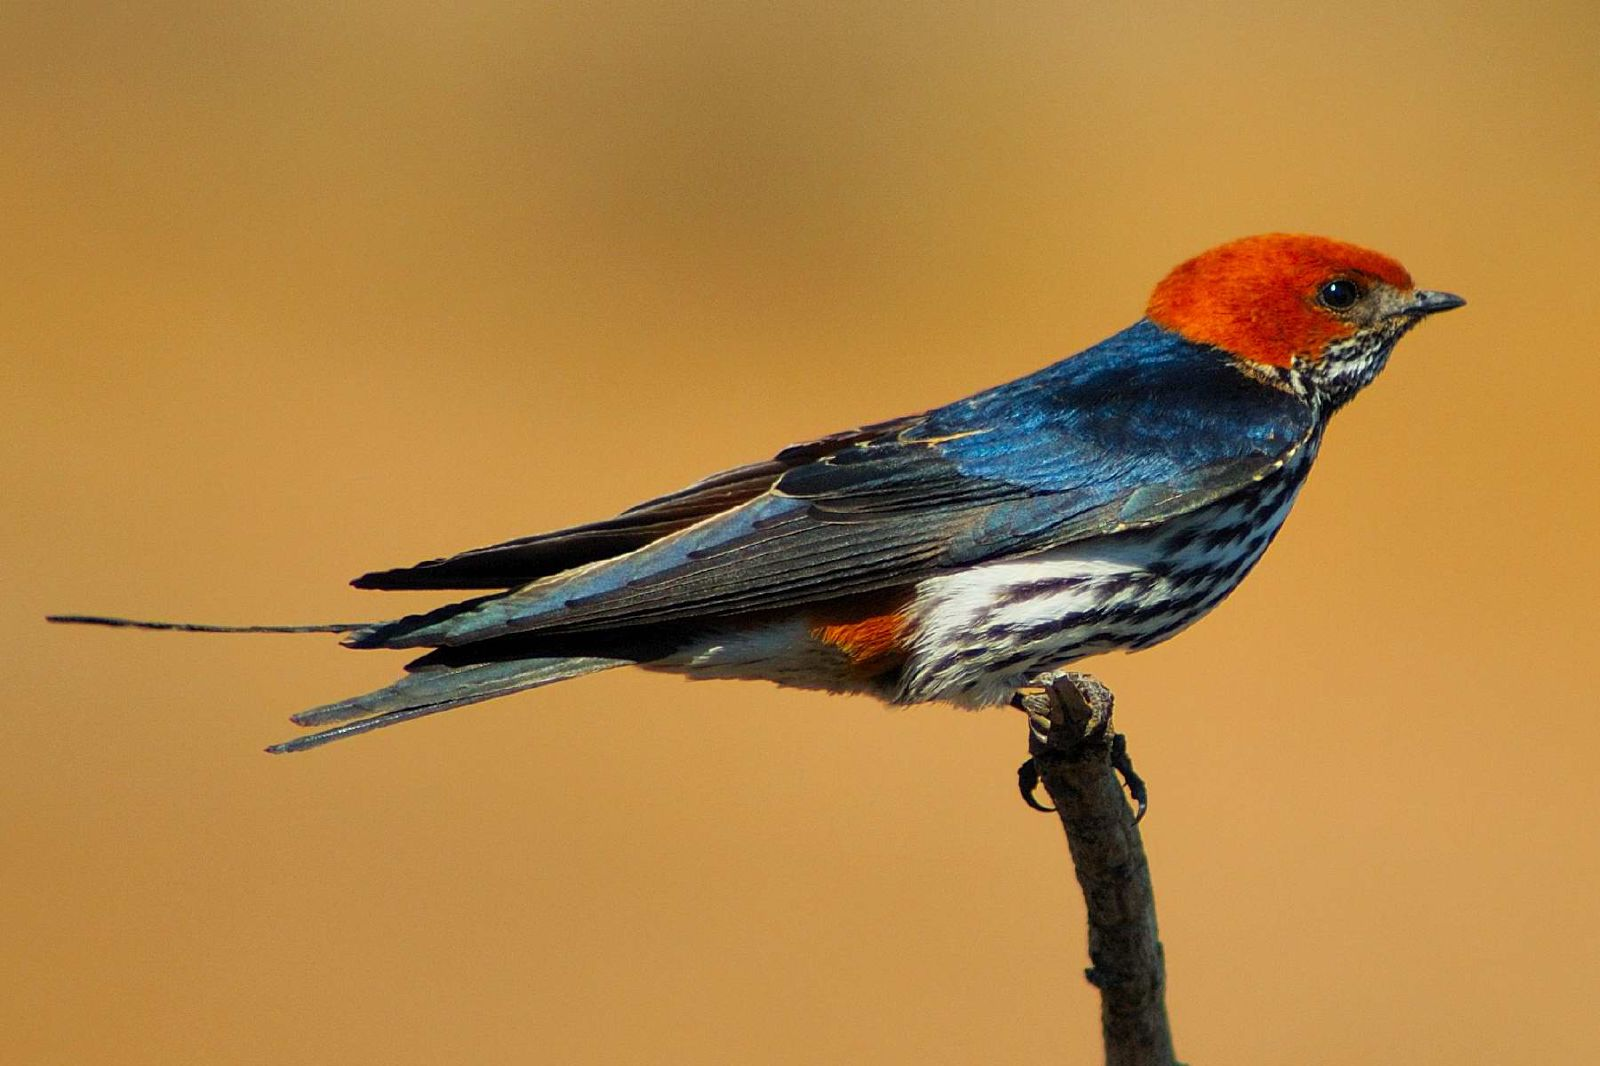
\includegraphics[width=0.5\columnwidth]{swallow.jpg} % Example image
\end{center}

%------------------------------------------------

\subsection*{Answer}

While this question leaves out the crucial element of the geographic origin of the swallow, according to Jonathan Corum, an unladen European swallow maintains a cruising airspeed velocity of \textbf{11 metres per second}, or \textbf{24 miles an hour}. The velocity of the corresponding African swallows requires further research as kinematic data is severely lacking for these species.

%----------------------------------------------------------------------------------------

\section*{Question 2}

\begin{problem}
	How much wood would a woodchuck chuck if a woodchuck could chuck wood?
	
	\medskip
	
	\begin{enumerate}[(\itshape a\normalfont)] % Sub-questions styled as italic letters
		\item Suppose ``chuck" implies throwing.
		\item Suppose ``chuck" implies vomiting.
	\end{enumerate}
\end{problem}

%------------------------------------------------

\subsection*{Answer}

\begin{enumerate}[(\itshape a\normalfont)] % Sub-questions styled as italic letters
	\item According to the Associated Press (1988), a New York Fish and Wildlife technician named Richard Thomas calculated the volume of dirt in a typical 25--30 foot (7.6--9.1 m) long woodchuck burrow and had determined that if the woodchuck had moved an equivalent volume of wood, it could move ``about \textbf{700 pounds (320 kg)} on a good day, with the wind at his back".
    
	\item A woodchuck can ingest 361.92 cm\textsuperscript{3} (22.09 cu in) of wood per day. Assuming immediate expulsion on ingestion with a 5\% retainment rate, a woodchuck could chuck \textbf{343.82 cm\textsuperscript{3}} of wood per day.
\end{enumerate}

%----------------------------------------------------------------------------------------

\section*{Question 3}

\begin{problem}
	Identify the author of Equation \ref{eq:bayes} below and briefly describe it in Latin.
	
	\medskip
	
	\begin{equation}\label{eq:bayes}
		P(A|B) = \frac{P(B|A)P(A)}{P(B)}
	\end{equation}
	
	\smallskip
\end{problem}

%------------------------------------------------

\subsection*{Answer} 

Lorem ipsum dolor sit amet, consectetur adipiscing elit. Praesent porttitor arcu luctus, imperdiet urna iaculis, mattis eros. Pellentesque iaculis odio vel nisl ullamcorper, nec faucibus ipsum molestie. Sed dictum nisl non aliquet porttitor. Etiam vulputate arcu dignissim, finibus sem et, viverra nisl. Aenean luctus congue massa, ut laoreet metus ornare in. Nunc fermentum nisi imperdiet lectus tincidunt vestibulum at ac elit. Nulla mattis nisl eu malesuada suscipit.

%----------------------------------------------------------------------------------------

\section*{Question 4 (bonus marks)}

\begin{problem}
	The table below shows the nutritional consistencies of two sausage types. Explain their relative differences given what you know about daily adult nutritional recommendations.
	
	\bigskip
    
	\begin{center}
		\begin{tabular}{l l l}
			\toprule
			\textit{Per 50g} & Pork & Soy \\
			\midrule
			Energy & 760kJ & 538kJ\\
			Protein & 7.0g & 9.3g\\
			Carbohydrate & 0.0g & 4.9g\\
			Fat & 16.8g & 9.1g\\
			Sodium & 0.4g & 0.4g\\
			Fibre & 0.0g & 1.4g\\
			\bottomrule
		\end{tabular}
	\end{center}
	
	\medskip
\end{problem}

%------------------------------------------------

\subsection*{Answer}

Lorem ipsum dolor sit amet, consectetur adipiscing elit. Praesent porttitor arcu luctus, imperdiet urna iaculis, mattis eros. Pellentesque iaculis odio vel nisl ullamcorper, nec faucibus ipsum molestie. Sed dictum nisl non aliquet porttitor. Etiam vulputate arcu dignissim, finibus sem et, viverra nisl. Aenean luctus congue massa, ut laoreet metus ornare in. Nunc fermentum nisi imperdiet lectus tincidunt vestibulum at ac elit. Nulla mattis nisl eu malesuada suscipit.

%----------------------------------------------------------------------------------------

\section*{Question 5 (bonus marks)}

\begin{problem}
	\lstinputlisting[
		caption=Luftballons Perl Script, % Caption above the listing
		label=lst:luftballons, % Label for referencing this listing
		language=Perl, % Use Perl functions/syntax highlighting
		frame=single, % Frame around the code listing
		showstringspaces=false, % Don't put marks in string spaces
		numbers=left, % Line numbers on left
		numberstyle=\tiny, % Line numbers styling
	]{luftballons.pl}
	
	\begin{enumerate}
		\item How many luftballons will be output by the Listing \ref{lst:luftballons} above?
		\item Identify the regular expression in Listing \ref{lst:luftballons} and explain how it relates to the anti-war sentiments found in the rest of the script.
	\end{enumerate}

\end{problem}

%------------------------------------------------

\subsection*{Answer}

\begin{enumerate}
	\item 99 luftballons.
	\item Lorem ipsum dolor sit amet, consectetur adipiscing elit. Praesent porttitor arcu luctus, imperdiet urna iaculis, mattis eros. Pellentesque iaculis odio vel nisl ullamcorper, nec faucibus ipsum molestie. Sed dictum nisl non aliquet porttitor. Etiam vulputate arcu dignissim, finibus sem et, viverra nisl. Aenean luctus congue massa, ut laoreet metus ornare in. Nunc fermentum nisi imperdiet lectus tincidunt vestibulum at ac elit. Nulla mattis nisl eu malesuada suscipit.
\end{enumerate}

%----------------------------------------------------------------------------------------

\end{document}
